%
%-----------------------------------
\newpage
\section{Narrow Line Magneto-Optical Trap}
%-----------------------------------
%

\begin{wrapfigure}{l}{0.4\textwidth}
    \centering
    \vspace{-10px}
    \caption{Atomic cloud shape in nMOTs for small laser intensities.}
    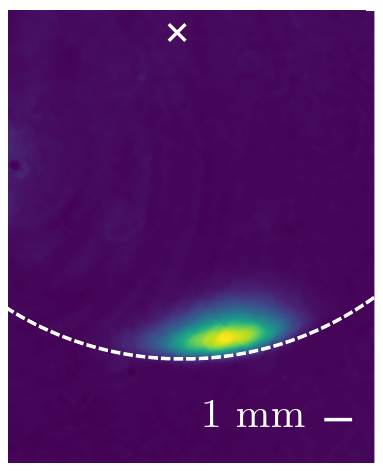
\includegraphics[width=0.3\textwidth]{USPSC-img/atomic_cloud_shape_in_nMOTs.png}
    \legend{Typical \textit{in situ} absorption image of an atomic sample in a nMOT. \\ Source: \cite{dreon2017optical}}
    \label{fig:atomic-cloud-shape-nMOTs}
    \vspace{-10px}
\end{wrapfigure}

In previous sections, we have been neglecting the gravity effect on the MOT parameters. This assumption is valid when the MOT force is much higher than gravity. The maximum radiation pressure force on an atom is $ \hbar k \Gamma / 2 $ from equation (\ref{eq:1D-MOT-force-components}). Therefore, the ratio between the maximum radiation pressure force and gravity is
\begin{equation}
    R \equiv \frac{\hbar k \Gamma}{2 m g},
\end{equation}
where $ m $ is the atomic mass and $ g $ is the gravitation acceleration. Usually, $ R $ is on the order of $ 10^5 $. Hence, the gravity force is negligible since the radiation pressure force is much higher. However, the smaller $ \Gamma $, the higher the gravity effect so that for $ \Gamma \sim\ \textrm{kHz} $, this ratio approaches values on the order of $ 10 $. In this case, the centre of mass moves towards the gravity direction such that, for small laser intensities, the atoms gather on the bottom of the surface of an ellipsoid, assuming a "bowl" shape as illustrated in figure \ref{fig:atomic-cloud-shape-nMOTs}.

Furthermore, $ \Gamma $ is also known as \textbf{scattering rate} since it defines the average number of photon scattering. Then, the lower $ \Gamma $, the lower the number of photon scatterings.

\textcolor{red}{Working on it. Topics that are being written:
\begin{enumerate}
    \item Discussion about the discrete momentum exchange
    \item Defining nMOTs and their three regimes
    \item Detailed analyses of the power-broadened regime on which we obtain the results in agreement with the experimental data
    \item Brief discussion about the quantum regime which won't be the focus
    \item Dysprosium and strontium as candidates to nMOTs
\end{enumerate}
}

%-----------------------------------
\subsection{Operating regimes}
\label{sec:nMOT-operating-regimes}
%-----------------------------------

%-----------------------------------
\subsection{Dysprosium and strontium nMOTs}
\label{sec:nMOT-operating-regimes}
%-----------------------------------
